\section{Problem-Analyse}\label{l:problemanalyse}

In diesem Kapitel werden die Probleme beschrieben, die bei der Erstellung von In"-for"-ma"-ti"-ons- und Kom"-mu"-ni"-ka"-ti"-ons"-me"-di"-en in Zusammenhang mit den dargestellten Texten auftreten. Abschnitt \ref{l:besondererolle} analyisiert die besondere Rolle von Text, anschließend zeigt Abschnitt \ref{l:officeprobleme} (S.\pageref{l:officeprobleme} ff.) typische Probleme auf, die im Verlauf von Projekten entstehen. Abschnitt \ref{l:praxisbeispiele} (S.\pageref{l:praxisbeispiele} ff.) belegt dies mit Beispielen aus der Praxis. 

\bigskip

Die Analyse des Problems basiert auf Interviews mit Personen, die in ihrem Arbeitsalltag regelmäßig mit Texten zu tun haben. Eine Liste der interviewten Personen findet sich in Tabelle \ref{table:interviewpartner} auf Seite~\pageref{table:interviewpartner}.

\subsection{Die besondere Rolle von Text in In"-for"-ma"-ti"-ons- und Kom"-mu"-ni"-ka"-ti"-ons"-me"-di"-en}\label{l:besondererolle}

Es existieren nahezu keine Medien, die ohne Texte auskommen, denn Text ist im Gegensatz zu Grafiken, Fotos oder Animationen ein eindeutiger Informationsträger und unterliegt viel weniger stark einer Interpretation durch den Rezipienten eines Mediums als die symbolisierte oder stilisierte Darstellung von Informationen in audiovisuellen Medien. Text wird in der Marketing-Kommunikation als Unterstützung der zu übermittelnden Information verwendet. Hat man die Aufmerksamkeit des Betrachter eines Produkts erlangt, liefert Text weitere Informationen zum Produkt, er dient dazu, die emotionale Botschaft zu erläutern und zu präzisieren. Auch aus rechtlichen Aspekten ist Text aus den genannten Gründen der einzige verbindliche Informationsträger -- bestes Beispiel hierfür ist das sogenannte \typoquotes{Kleingedruckte}, dass sich gerade bei inhaltlich sehr stark komprimierten Werbeformen, wie z.B. Plakat- oder Fernsehwerbung, findet. Ist die Textmenge, die in der Marketing-Kommunikation zum Einsatz kommt, noch überschaubar, gibt es doch Medien die hauptsächlich aus Text bestehen. Hierunter fallen klassische Druckerzeugnisse wie Broschüren und Kataloge oder Produkte der Unternehmenskommunikation wie Jahresberichte und Pressemeldungen. Besonders digitale Medien werden oft mit großen Textmengen versehen -- von der einfachen Produkt-Microsite, über Werbemittel wie Newsletter bis zur Unternehmenswebsite -- die Möglichkeit Inhalte hierarchisch zu strukturieren und sogar über eine Suche zugänglich zu machen hebt eine Limitierung des Umfanges, wie bei Druckprodukten, praktisch auf.

\begin{figure}[htb]
\begin{center}
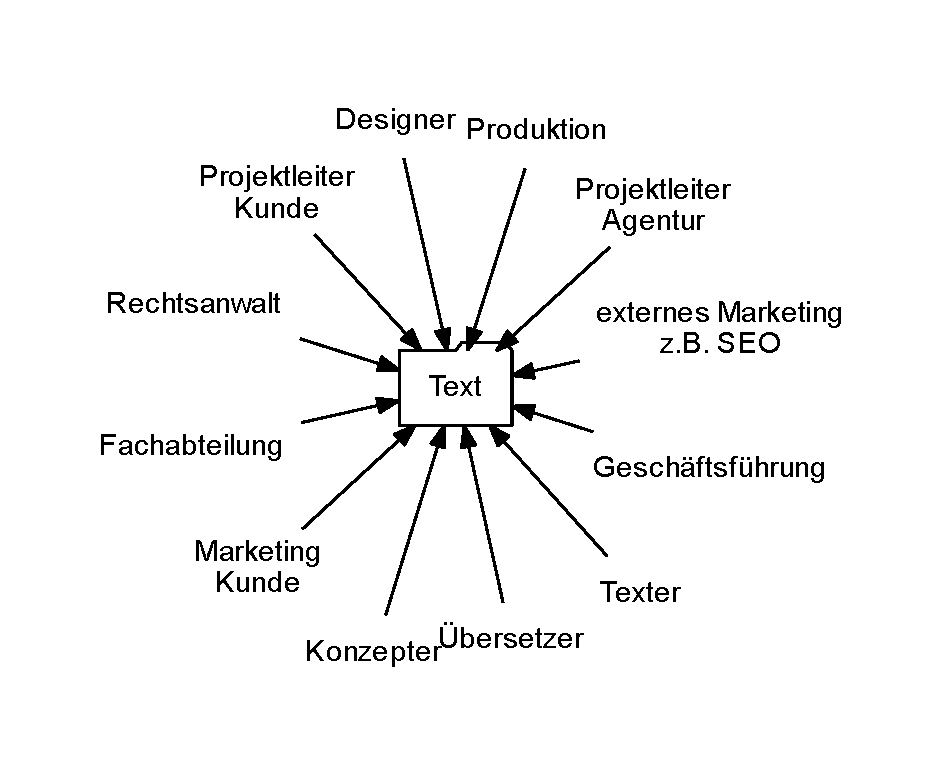
\includegraphics[width=\textwidth]{media/chart-2.pdf}
\end{center}
\caption{Bei der Erstellung von Texten beteiligte Personen}
\label{chart:2}
\end{figure}

Betrachtet man die Abläufe von Projekten, in deren Verlauf Medien erstellt werden, lassen sich bezüglich der Textbestandteile dieser Produkte immer wieder sehr ähnliche Vorgehensweisen und Besonderheiten beobachten. Aufgrund der verbindlichen Natur von Text sind an der Erstellung der Texte für das Medium mehr Personen beteiligt, als es z.B. für die Gestaltung, der Auswahl von Bildmaterial oder für die Programmierung der Fall ist,  da Text sehr viele verschieden Kriterien erfüllen muss. Tabelle \ref{table:textkriterien} (S.\pageref{table:textkriterien}) listet exemplarisch eine typische Gruppe von Personen auf, die im Verlauf des Projektes Einfluss auf den Text eines Produktes haben. Dieser Einfluss wird dabei in der Regel nicht in einer sinnvollen Reihenfolge und im Sinne des geplanten Projektverlaufes ausgeübt. Gerade auf die Mitarbeiter auf Kundenseite haben Agenturen keinen Einfluss; in Projektplänen lassen sich zwar verbindliche Termine für die Lieferung von Texten des Kunden festlegen, dies verhindert aber keinesfalls, dass zu einem späteren Zeitpunkt Änderungen notwendig werden -- Hinweise von Anwälten sollten im besten Fall \emph{vor} einer Übersetzung vorliegen, richtet sich aber nach ihren eigenen Terminplänen. Auch die Kriterien wie Text beeinflusst wird, sind sehr vielfältig: Im Entwurf und in der Umsetzung der Produkte legen Designer, Architekten und Produzenten die Struktur von Text wie Art der Ansprache, maximale Wortlänge, Anzahl der Wörter einer Überschrift fest oder diese werden durch das verwendete Medium vorgegeben, Texter legen die Inhalte fest, die wiederum durch Wünsche des Kunden beeinflusst werden; das Lektorat, Fachabteilungen und Anwälte begutachten die Texte dann bezüglich der jeweils erforderlichen Korrektheit.

\TODO : Die Trennung zwischen Intern und Extern ist nur exemplarisch. Sie ist flexibel und je nach Projekt unterschiedlich.

\begin{table}
\begin{center}
\begin{tabular}{@{}l l l l}
\textbf{Kriterium} & \textbf{Art} & \textbf{Verantwortlich} & \textbf{Organisation}\\
\hline
Aufgabenverteilung & Mitarbeiter & Projektleiter & Agentur\\
\hline
Zielgruppe & Struktur & Informationsarchitektur & Agentur\\
\hline
Umfang, Satzlänge & Struktur & Art-Direktion & Agentur\\
\hline
Länge einzelner Wörter & Struktur & Programmierer & Agentur\\
\hline
Information & Inhalt & Texter & Extern\\
\hline
Orthographie & Korrektheit & Lektorat & Extern\\
\hline
Übersetzung & Sprache & Übersetzungsbüro & Extern\\
\hline
Suchmaschinen-Optimierung & Inhalt & SEO-Experte & Extern\\
\hline
Aufgabenverteilung & Mitarbeiter & Projektleiter & Kunde\\
\hline
Fachliche Aspekte & Korrektheit & Fachabteilung & Kunde\\
\hline
Rechtliche Aspekte & Korrektheit & Rechtsanwalt & Kunde\\
\hline
Werbeaussagen & Inhalt & Marketingabteilung & Kunde\\
\hline
… & … & …
\end{tabular}
\caption{Kriteren von Textbausteinen und verantwortliche Personen}
\label{table:textkriterien}
\end{center}
\end{table}

Wie man Tabelle \ref{table:textkriterien} entnehmen kann, existieren vielfältige Einflussmöglichkeiten auf die Gestaltung von Texten für Medien die sich auf viele Verantwortliche verteilen. Der Grund dafür ist, dass alle Beteiligten jeweils spezifisches Fachwissen in den Text einfließen lassen, seien es gestalterische Aspekte, die Einfluss auf die Struktur haben, oder das wissen über exakte technische Abläufe, die nur Spezialisten in den Fachabteilungen auf Kundenseite bekannt sind. Dieses Expertenwissen kann nicht für die meist kurze Projektlaufzeit an die umsetzenden Agentur vermittelt werden. Es ist also unvermeidlich, dass Text während des gesamten Projektverlauf geändert werden kann. Neben den Einflüssen durch Experten gibt es auch projektbedingte Einflüsse auf Text in letzter Minute. Sind in Texten Informationen enthalten sind, die einen zeitlichen Aspekt abbilden, ergeben sich durch Verzögerungen im Projekt automatisch Änderungsanforderungen. Ein Beispiel sind Gewinnspiele: Verschiebt sich durch Probleme während dem Projekt der Zeitpunkt, ab dem ein Produkt beim Rezipienten vorliegt, müssen auch eventuell knapp kalkulierte Gewinnspieltermine angepasst werden. Ein weiterer Grund für vielfältige Textänderungen im Verlauf eines Projektes ist die Erwartungshaltung des Kunden -- da es Kunden aus ihrem eigenen Arbeitsalltag gewöhnt sind, mit Textverarbeitungsprogramme zu arbeiten, und sie so aus eigener Erfahrung vermeintlich wissen dass Texte schnell geändert sind, erwarten sie auch, dass die Texte im Produkt bis zum Schluss geändert werden können; ihnen ist nicht bewusst, das vom ursprünglichen Text im Quelldokument bis zur Darstellung im fertigen Produkt viele aufwändige Arbeitsschritte nötig sein können.

\subsection{Das Werkzeug der Wahl zur Verwaltung von Text: \trademark{Word} und \trademark{Excel}}

Zur Abbildung der komplexen Abläufe bei der Erstellung von In"-for"-ma"-ti"-ons- und Kom"-mu"-ni"-ka"-ti"-ons"-me"-di"-en liefern etablierte Software-Hersteller passende Lösungen auch speziell für Texte: Mit \trademark{InCopy} liefert \trademark{Adobe} eine \citequotes{Lösung für Texterstellung und -bearbeitung, die aufgrund der engen Integration mit Adobe InDesign® CS5.5 effektivere Zusammenarbeit zwischen Redakteuren und Layoutern ermöglicht} \cite{adobeincopy} und  die \trademark{Content Station} von \trademark{Woodwing} \citequotes{ist […] eine einzige Oberfläche für alle Schritte des Publishing-Prozesses. […] Unter Nutzung der Desktop- oder der Web-Version können die Team-Mitglieder unabhängig ihres Aufenthaltsorts mitarbeiten} \cite{woodwing} -- um nur zwei Beispiele zu nennen. Doch obwohl spezialisierte Werkzeuge existieren findet man diese in Agenturen nur selten -- das Werkzeug der Wahl zur Verwaltung der Texte ist in der Regel eine in der Agentur vorhandene Textverarbeitungs- oder Tabellenkalkulationssoftware, in den allermeisten Fällen handelt es sich dabei um den Marktführer in diesem Bereich: \trademark{Microsoft} \trademark{Word} oder \trademark{Excel}. Auf die Probleme, die durch deren Einsatz entstehen wird im nachfolgenden Abschnitt \ref{l:officeprobleme} (S.\pageref{l:officeprobleme}) eingegangen. Zu erst muss jedoch erst untersucht werden, warum statt spezieller Werkzeuge, die für den komplizierten Workflow in Projekten entwickelt wurden, \trademark{Word} oder \trademark{Excel} eingesetzt werden.

\bigskip

Oberflächlich betrachtet, bieten Textverarbeitungsprogramme die notwendigen Funktionen, um Texte zu verwalten und sind damit scheinbar die natürliche Wahl. Die verwendeten Funktionen sind dabei nachfolgend beschrieben.

\begin{figure}[htb]
\begin{center}
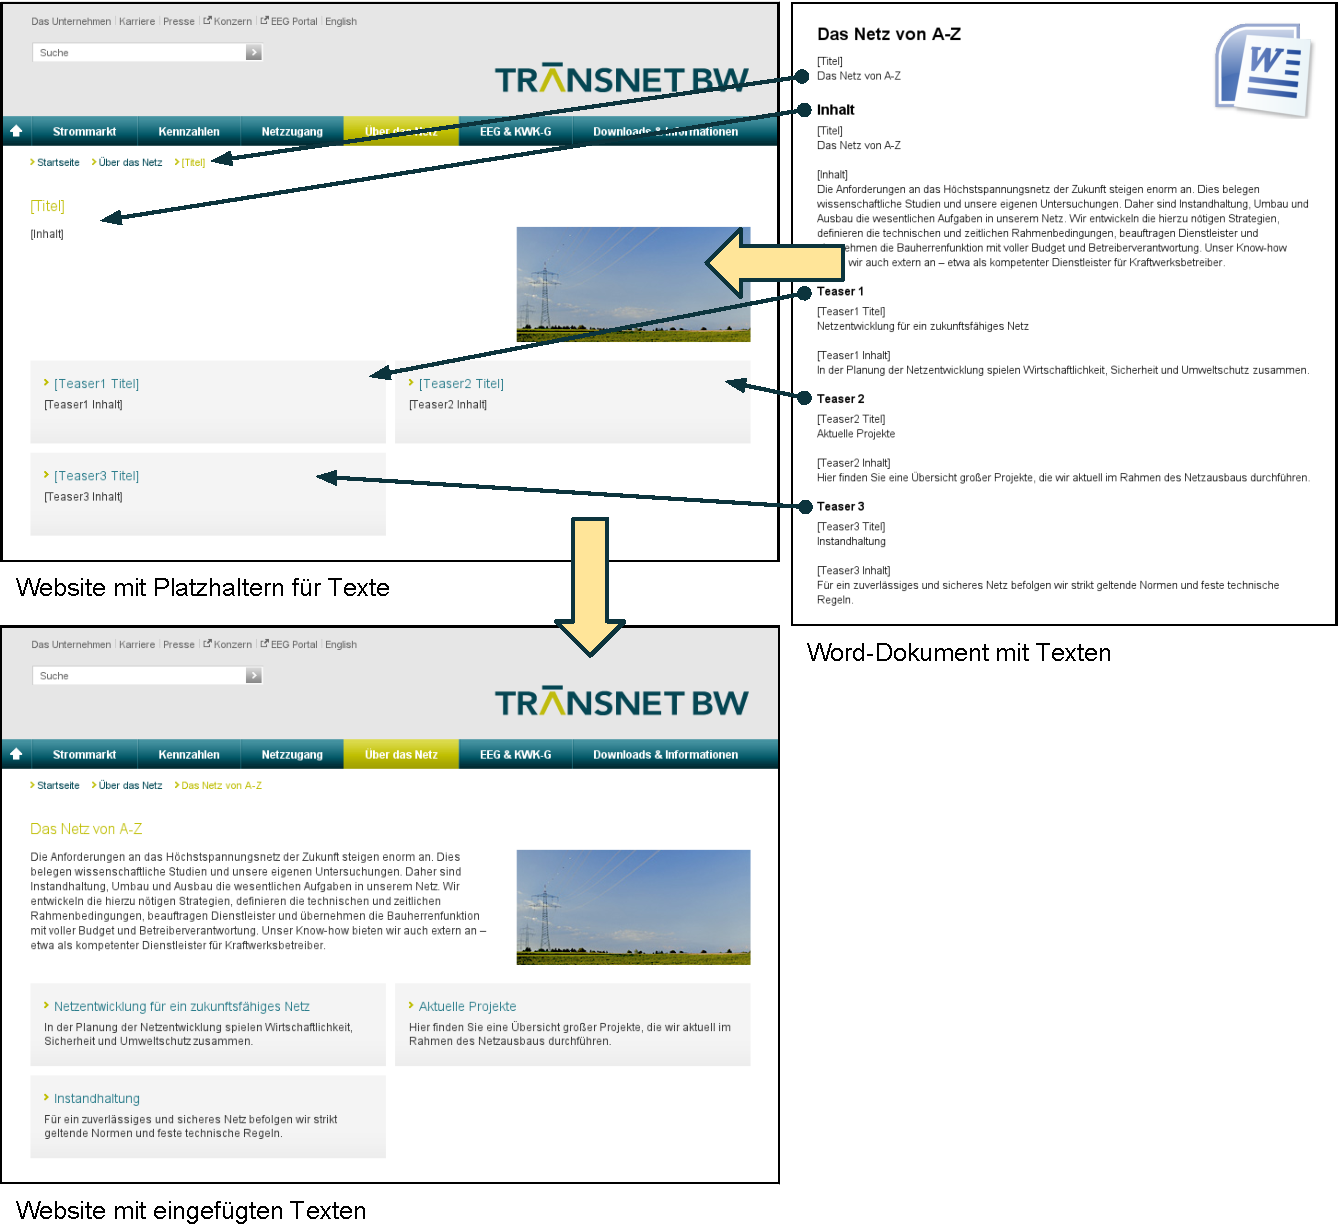
\includegraphics[width=\textwidth]{media/Textbooklet-Word-Dokument.pdf}
\end{center}
\caption{\trademark{Word}-Dokument mit Texten für eine Internetseite}
\label{f:wordbooklet}
\end{figure}

\begin{figure}[htb]
\begin{center}
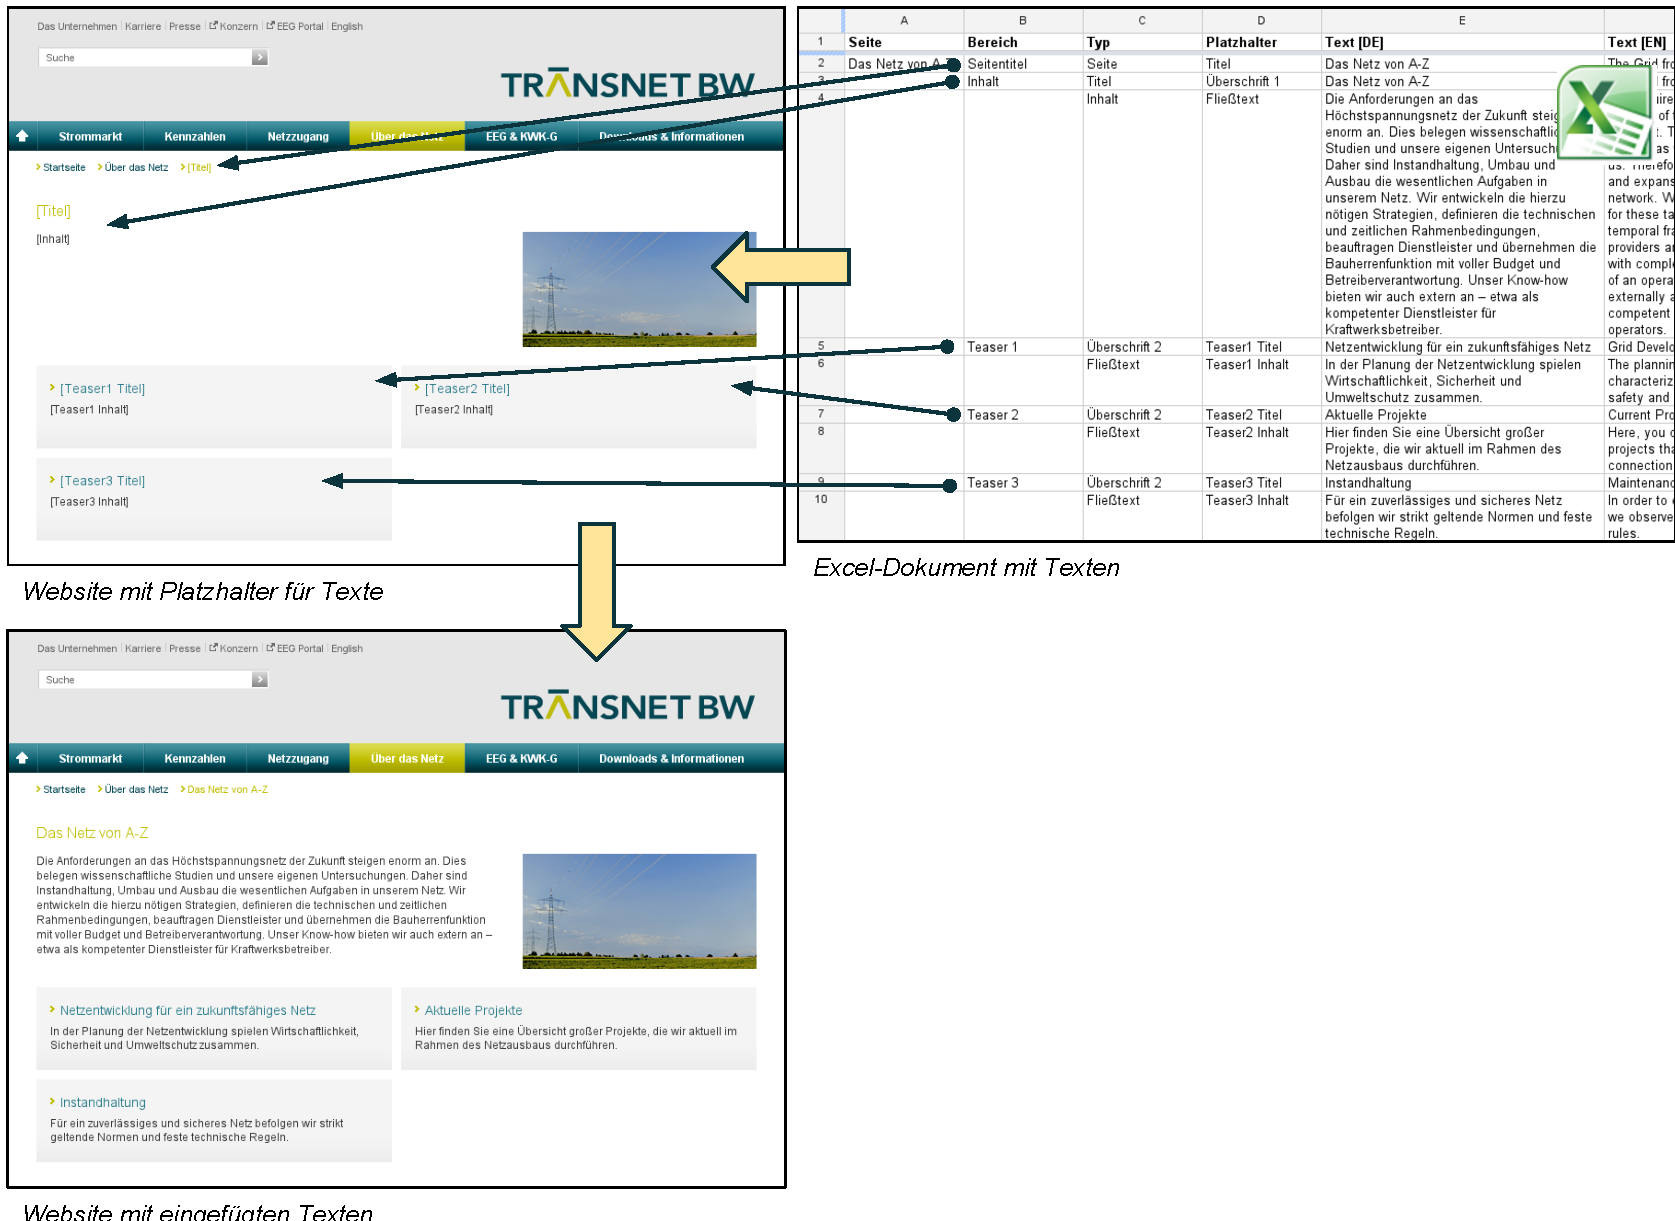
\includegraphics[width=\textwidth]{media/Textbooklet-Excel-Dokument.pdf}
\end{center}
\caption{\trademark{Excel}-Dokument mit Texten für eine Internetseite}
\label{f:excelbooklet}
\end{figure}

\paragraph{Strukturierung von Texten} Die Möglichkeit, Texte hierarchisch in Dokumente, Seiten, Kapitel, Abschnitte oder Absätze zu unterteilen ermöglicht es die Textbausteine für ein Produkt geordnet zu Erfassen. Neben den eigentlichen Texten lassen sich dazu auch Zusatzinformationen wie die Klasse des Textes dort zuzuordnen. Abbildung~\ref{f:wordbooklet} (S.\pageref{f:wordbooklet}) zeigt beispielhaft ein \trademark{Word}-Dokument, in dem die Texte für eine Website definiert werden. Im Dokument existiert pro Seite der Internetpräsenz jeweils ein Abschnitt, der alle Texte auf der Seite beschreibt. Dort finden sich die Texte zu den Platzhaltern, die in der Website verwendet werden, die dann an deren Stelle eingefügt werden. Über die Formatierung der Überschriften wird die Hierarchie der Texte definiert. Die Verwendung von Tabellen statt Dokumenten ist eine weitere Möglichkeit die verwendeten Texte zu erfassen. Abbildung~\ref{f:excelbooklet} (S.\pageref{f:excelbooklet}) zeigt beispielhaft ein \trademark{Excel}-Dokument, in dem pro Zeile ein Text definiert wird. In den Spalten findet sich neben dem eigentlichen Text Zusatzinformationen wie z.B. die Text-Klasse. Tabellarische Dokumente werden oft bei umfangreichen Projekten oder um mehrere Sprachversionen zu verwalten verwendet.

\paragraph{Rechtschreibkorrektur} In Textverarbeitungsprogrammen sind ausgefeilte Funktionen zur Rechtschreibkorrektur enthalten, die bereits während der Eingabe auf Fehler aufmerksam machen und für viele Sprachen verfügbar sind. So ist sichergestellt, dass bereits die erste Version eines Textes relativ wenige Fehler enthält.

\paragraph{Kommentare} Es ist möglich in \trademark{Word}- und \trademark{Excel}-Dokumenten Kommentare zu hinterlassen. Diese werden gesondert hervorgehoben und können zum Austausch über den Text oder für Hinweise zur Verwendung hinterlegt werden und von allen Bearbeitern eingesehen werden.

\paragraph{Änderungsverfolgung} Wenn die Änderungsverfolgung aktiviert ist, werden alle Änderungen an einem Dokument aufgezeichnet. Diese Information kann dabei helfen, mehrere Versionen eines Dokumentes manuell zusammenzuführen oder Änderungen an Inhalten vorzuschlagen, zu prüfen und selektiv zu übernehmen.

\paragraph{Verzeichnisse} In \trademark{Word}-Dokumenten ist es möglich, Verzeichnisse wie z.B. ein Inhaltsverzeichnis anzulegen. Dies hilft dabei, bei größeren Projekten einen Überblick über den Aufbau des Produktes zu erhalten, sofern die Inhalte mit den passenden Formatvorlagen versehen wurden.

\paragraph{Suchen \& Ersetzen} Da sich die Texte in einem großen Dokument befinden können mit den Funktionen zum Suchen \& Ersetzen schnell bestimmte Inhalte gefunden und angepasst werden.

\paragraph{Export} Die \trademark{Office}-Programme verfügen über die Möglichkeit des Exports in verschiedene Formate. Verwendet werden vor allem PDF bei \trademark{Word}-Dokument zur Abstimmung, unter andere auch deswegen, weil es in \trademark{Adobe} \trademark{Acrobat} umfangreiche Korrekturfunktionen gibt, und CSV in \trademark{Excel}, das möglich macht die Text mit Hilfe von speziellen Programmen in andere Systeme zu importieren.

\paragraph{Formatierungsfunktionen} Mit umfangreiche Formatierungsfunktion ermöglichen zusätzliche Informationen zu Texten zu hinterlegen. Oft werden durch farbige Markierung Passagen markiert, die zu überarbeiten sind, entfallen oder inhaltlich überarbeitet werden müssen. Auch können Formatieren so angelegt sein, dass sie in das Produkt übernommen werden sollen -- in der Regel werden dann Teile des oder einzelne Wörter Textes fett oder kursiv formatiert. Funktionen zum Setzen von Hyperlinks werden gerade bei Web-Projekten verwendet um Links zu definieren, die im Produkt verwendet werden sollen.

\bigskip

Auch im Hinblick auf nicht-funktionale Aspekte bieten Textverarbeitungsprogramme einige Vorteile, sind sie doch in den allermeisten Unternehmen der Standard zur Textverarbeitung und sogar plattformunabhängig verfügbar -- zumindest existiert die Möglichkeit das \trademark{Microsoft Office}-Dateiformat auf allen Plattformen zu bearbeiten. Da bei allen Projektbeteiligten eine Installation von \trademark{Microsoft Office} vorausgesetzt werden kann, werden \trademark{Word} und \trademark{Excel} zu \typoquotes{leichtgewichtigen} Werkzeugen, das vom vom Anwender keine zusätzlichen Aufwände, z.B. bei der Installation oder Eingewöhnung, abverlangen. Selbst auf Plattformen die von \trademark{Microsoft Office} nicht offiziell unterstützt werden, wie z.B. Linux, existieren Programme mit denen das Office-Dokumenten-Format geöffnet und bearbeitet werden kann, unter Linux ist dies z.B. \trademark{Libre Office}. Da \trademark{Office}-Dokumente in nur einer Datei gespeichert werden, sind diese einfach auszutauschen -- in Agenturen werden die Dateien in der Regel auf einem Netzwerk-Laufwerk gespeichert, unternehmensfremde Mitarbeiter erhalten die Dateien via E-Mail, FTP-Server oder Filesharing-Anbieter, z.B. Dropbox. So wird das gemeinsame Arbeiten an den Texten, zumindest nacheinander, möglich. 

\bigskip

Wie in diesem Abschnitt gezeigt wurde, sind Textverarbeitungs- und Tabellenkalkulationsprogramme wie \trademark{Microsoft} \trademark{Word} und \trademark{Excel} nominell für den Einsatz zur Verwaltung von Texten für Medien geeignet. Dies erklärt, warum sie zu Beginn eines Projektes als geeignet angesehen und in Agenturen immer wieder als Werkzeug für die Erfassung, Definition und Übersetzung der Texte eines Projektes ausgewählt werden. Im alltäglichen Gebrauch treten jedoch Probleme gerade im Bereich des gemeinsamen Bearbeitens, paralleler oder nachträglicher Änderungen und der Übertragung der fertigen Texte in den Produktionsprozess auf, die im folgenden Abschnitt erläutert werden.

\subsection{Probleme bei der Verwendung von Textverarbeitungs- und Tabellenkalkulationsprogrammen im Verlauf eines Projektes}
\label{l:officeprobleme}

Wie im vorangegangenen Abschnitt gezeigt wurde, sind Textverarbeitungs- und Tabellenkalkulationsprogramme wie \trademark{Microsoft} \trademark{Word} und \trademark{Excel} der Standard für die Verwaltung von Texten in Projekten zur Erstellung für In"-for"-ma"-ti"-ons- und Kom"-mu"-ni"-ka"-ti"-ons"-me"-di"-en. In den für diese Bachelor-Thesis geführten Interviews haben jedoch alle Personen von vielfältige Problemen in Zusammenhang mit diesen Programmen berichtet. Dies belegt zum einen, dass am gängigen Workflow viele Möglichkeiten zur Verbesserung existieren und liefert zum andere auch Hinweise, wie der verbesserte Workflow im Detail gestaltet werden muss. In diesem Abschnitt werden die beobachteten Probleme beschrieben.

\label{p:serielles-konzept}\paragraph{Serielles Bearbeitungskonzept} Das grundsätzliche Bearbeitungskonzept, das in \trademark{Word} und \trademark{Excel} zum Einsatz kommt ist seriell, das bedeutet, dass eine Dokument gleichzeitig nur von einer Person bearbeitet werden kann. Soll mit mehreren Personen an einem Dokument gearbeitet werden, muss dieses zwischen allen Beteiligten ausgetauscht werden. Dies geschieht, in dem die Dokumenten-Datei entweder per E-Mail jeweils zum nächsten Bearbeiter verschickt wird oder die Datei auf ein, durch alle Beteiligten erreichbaren Speicherplatz verschoben werden. In Agenturen handelt es sich hierbei meistens um eine Netzwerklaufwerk -- hierauf haben aber nur die im lokalen Netzwerk integrierten Mitarbeiter Zugriff. Soll die Datei auch externen Mitarbeitern oder dem Kunden zur Verfügung gestellt werden, werden diese wieder per E-Mail verschickt oder in extern erreichbare Speicherort kopiert, wie z.B. FTP-Server, Wikis und Extranet-Portale oder es kommen spezielle Programme zum Dateiaustausch zum Einsatz, wie z.B. \trademark{Dropbox}. Die Organisation dieses Austausches ist besonders dann aufwändig, wenn Dateien sich nicht mehr unter Kontrolle der Agentur befinden, weil sie z.B. zum Kunden zur Kontrolle geschickt wurden. Dann kommt es dazu, dass mehrere Versionen des Dokumentes parallel existieren: eine Version beim Kunden, die dort mit Änderungen und Ergänzungen versehen wird und eine Version in der Agentur in der sich aufgrund von Änderungen im Verlauf des Projekts Text ändern. Um anschließend alle Beteiligten auf den aktuellen Stand zu müssen die verschiedenen Versionen des Dokumentes manuell zusammengeführt werden -- automatisiert ist das mit \trademark{Word} und \trademark{Excel} nicht möglich. Neben dem zeitlichen Aufwand birgt das manuelle Zusammenführen weitere Fehlerquellen, da Änderungen an Texten durch Copy\&Paste übertragen werden, kann es gerade bei großen Dokumenten passieren, dass man die Änderungen an der falschen Stelle einarbeitet, sofern im Dokument sich ähnelnde Textabschnitte existieren. Aus Kostengründen und weil es sich dabei um eine repetitive Arbeit handelt ist es nicht selten der Fall, dass diese Änderungen von Praktikanten oder studentischen Aushilfen durchgeführt werden, die mangels inhaltlicher Kenntnis den Zusammenhang der Text nicht kennen, was ebenfalls die irrtümliche Änderungen am Text durch fehlerhaftes Copy\&Paste begünstigt. Auch ist die Eindeutigkeit der Dateiversionen nicht gewährleistet, allein aufgrund des Zeitstempels kann keine genaue Aussage darüber getroffen werden, welche Datei die neueste ist. So muss man sich auf ein Benamungsschema für Dateien einigen, das im besten Fall klar erkennen lässt \emph{welches} Dokument das neueste ist. Üblich sind dabei Ergänzungen des Dateinamens mit Datumsinformationen, wie z.B. \texttt{Text\_Online\_2012-04-13.docx}. Folgen nicht alle Beteiligten diesem Schema, weil diese z.B. nicht ausreichend informiert sind, oder kommt es zu gleichzeitiger Änderungen von zwei Personen kann es so auch zu zwei verschiedenen Dateien mit dem gleichen Dateinamen kommen. Durch die Verteilung der Dokumente an verschiedene Speicherorte kommt es zu Situationen, in denen nicht klar ist, wer aktuell die \emph{neueste} Dateiversion hat. 

Tatsächlich existiert mit dem \trademark{Microsoft} \trademark{SharePoint}, einer Software für Intra-, Extra- und Internetportale, eine Lösung, die diese Probleme behebt \cite{sharepoint-shared-documents}. Mit Hilfe von \trademark{Shared Documents} lassen sich Dokument zentral ablegen. Sollen diese editiert werden, müssen Sie von der jeweiligen Person \typoquotes{ausgecheckt} werden, dies sperrt den Zugriff auf das Dokument durch andere Mitarbeiter. Sobald das Bearbeiten abgeschlossen wurde, wird die Datei wieder \typoquotes{eingecheckt}. So wird sichergestellt, dass es nie zwei Versionen der Datei mit unterschiedlichen Änderungen gibt. Diese Funktion behebt aber nicht den Umstand, das an einem Dokument immer nur eine Person arbeiten kann. Des weiteren ist \trademark{SharePoint} im Agen"-tur-Um"-feld kaum anzutreffen, was dem Umstand geschuldet ist, dass der Betrieb einer \trademark{SharePoint}-Instanz mit hohen Lizenz- und Personalkosten verbunden ist. Zum anderen setzen die Funktionen zum gemeinsamen Bearbeiten von \trademark{Word} oder \trademark{Excel} voraus, dass alle Mitarbeiter über die neuesten Programm-Version verfügen \cite{sharepoint-wordversions}. Dies kann aber auf Kundenseite nicht vorausgesetzt werden. Aufgrund der unterschiedlichen Programm-Versionen aber auch unterschiedlicher Betriebssystemen, kommt es beim Austausch der Dateien zu verschiedenen Kompatibilitätsproblemen, da in Agenturen meistens \trademark{Mac OS} verwendet wird, auf Kundenseite jedoch \trademark{Windows} verbreitet ist.

\paragraph{Monolithische Dokumente} Das Zusammenführen aller Textbausteine eines Produktes in einem Dokument hat den Nachteil, dass diese nur als Ganzes weitergeben werden können. In bestimmten Konstellationen ist es aber notwendig, sicherzustellen, dass bestimmte Inhalte nicht von allen Projektbeteiligten einsehbar sind. Zum einen kann es sich dabei um Informationen handeln, die der Geheimhaltung unterliegen oder sensibel sind, so dass sie nur bestimmten Personen zugänglich sein dürfen. Zum anderen kann es aus Kostengründen sinnvoll sein, die Prüfung von Texten durch Anwälte, oder die Übersetzung von Texten auf bestimmte Bereiche einzuschränken. In diesen Fällen wird es notwendig, verschieden Versionen des Dokumentes anzulegen, die an den jeweiligen Personenkreis angepasst sind. Dies erzeugt die Problem, die im vorangegangenen Abschnitt beschrieben wurden.

\paragraph{Feedback} Durch das Verteilen der Dokumente auf verschiedene Speicherorte wird eine parallele Kommunikation des Arbeitsstandes mittels E-Mail nötig, bei der jeweils dem nächsten Bearbeiter mitgeteilt wird, dass er mit seiner Aufgabe weiter fortfahren kann. Der Ablauf und die Reihenfolge der Kommunikation ergibt sich durch die Aufgaben der beteiligten Personen, aber auch durch informelle Absprachen. Gerade zwischen Agentur und Kunden gibt es häufig \typoquotes{Flaschenhälse}, die zu Verzögerungen führen. Dies sind in den meisten Fällen die jeweiligen Projektleiter und Ansprechpartner, die auch bei technischen oder inhaltlichen Fragen jeweils der alleinige Empfänger sind, die Anfrage entgegen nehmen in in ihrem Unternehmen an die zuständige Person weiterleiten, auf deren Antwort warten um dann die Antwort zurück zu spielen. Hierdurch bilden sich umfangreiche und langlebige E-Mail-Kommunikationsketten, an denen viele, meistens zu viele, Personen beteiligt sind und in ungeordneter Reihenfolge Feedback liefern.

\paragraph{Strukturierung von Dokumenten} Eine der Gründe, warum \trademark{Word} und \trademark{Excel} zur Standardausstattung auf jedem Büro-Computer gehören, ist der, dass sie für einen sehr breiten Anwendungsbereich entwickelt wurden. Dies hat jedoch zur Folge, dass es mit einigem Aufwand verbunden ist, die passende Struktur für die Inhalte eines Produktes in einem Text- oder Tabellen-Dokument anzulegen. Hierbei wird meistens eine hierarchische Struktur mit Hilfe von Abschnitten angelegt (vgl. Abb. \ref{f:wordbooklet}, S.\pageref{f:wordbooklet}). In \trademark{Excel} wird im Hinblick auf die kompaktere Darstellung meisten aus besonderer Formatierungen verzichtet und mit sich wiederholenden Zellen gearbeitet (vgl. Abb. \ref{f:excelbooklet}, S.\pageref{f:excelbooklet}), die eine hierarchische Struktur simulieren -- die zweidimensionale Tabellendarstellung ist für komplexere Hierarchien nicht ausgelegt. Dies aufwändige Strukturierung des Dokuments muss auch geschehen, damit sich alle Anwender in den Dokumenten zurecht finden und eine eindeutige Zuordnung zwischen Textbausteinen im Dokument und den dafür vorgesehen Platzhaltern im fertigen Produkt möglich ist. Da beide Programme für diese Aufgabe keinerlei Vorlage und Unterstützung liefern, muss hier viel Arbeit investiert werden, die zudem noch vorausschauend genug sein muss, damit es im späteren Verlauf des Projektes durch nicht berücksichtige Fälle nicht notwendig wird, das Dokument komplett zu überarbeiten.

\paragraph{Formatierung} Die Formatierung der Textbausteine nach gestalterischen Aspekten, also das Hinzufügen von z.B. Hervorhebungen, Unterstreichungen und Absätzen wird zum Teil schon während der Erstellung der Texte vorgenommen. Hierbei werden die jeweiligen Funktionen der von \trademark{Word} und \trademark{Excel} verwendet. Ist dies in \trademark{Word} komfortabel möglich, sind die Möglichkeiten in \trademark{Excel} deutlich eingeschränkt. Hier lassen sich Zeichen-Formatierungen wie Hervorhebung, Farbe o.ä. nicht auf einzelne Worte oder Zeichen anwenden, sondern nur auf eine ganze Zelle. Auch Zeilenumbrüche stellen ein Problem dar. Diese sind zwar grundsätzlich möglich, jedoch kann es mangels Wissen dazu kommen, dass ein Bearbeiter einen Zeilenumbruch nicht innerhalb einer Zelle einfügt, sondern statt dessen eine neue Zeile einfügt. Werden die Zeilennummern oder bestimmte Spalten als Referenz-Schlüssel für den Text verwendet, führt das dazu, dass die zweite Zeile des Texte, nicht mehr zugeordnet werden kann um im Produkt fehlt. Werden Tabellen in \trademark{Word}-Dokumenten verwendet um z.B. tabellarische Inhalte in einem Produkt zu beschreiben, führt die aufgrund der beschränkten Seitengröße eines Textdokuments dazu, dass Tabellen mit vielen Spalten nur mit sehr kleinem Text dargestellt werden können, was das Bearbeiten der Texte schwierig macht. Üblich ist auch das Einfügen von Bildern, dies ist nötig, um die Zuordnung der Texte zu Produkten zu erleichtern oder um Untertitel Fotos zu definieren, hierbei treten dann zusätzliche Formatierungsproblem auf, da das platzieren von Bildern nur in beschränktem Maße beeinflusst werden kann. Problematisch ist auch der Austausch der Formatierungen zwischen verschieden Versionen von \trademark{Word} oder \trademark{Excel}, besonders wenn Dokumente von neueren Versionen in älteren Versionen angezeigt und bearbeitet werden, und vor allem dann, wenn die Dokumente in anderen Textverarbeitungs- und Tabellenkalkulationsprogramm wie z.B. \trademark{Apple} \trademark{iWorks} oder \trademark{LibreOffice} bearbeitet werden. Diese Programme unterstützen zwar \emph{per se} den Ex- und Import von \trademark{Microsoft}-Dateiformaten, bei der Konvertierung entstehen gerade bei Übertragen dieser Formatierungen  Unsauberkeiten. Sollen die Formatierungen dann in das Produkt übernommen werden kann dies nicht automatisch geschehen, da es für die verwendete Auszeichnungen keinen Standard gibt, der in allen Umgebungen verwendet werden kann. Deswegen müssen alle Formatierung manuell im Produkt angelegt werden, dies kann, ähnlich wie bei Copy\&Paste, zu Übertragungsfehlern führen.

\paragraph{Feedback und Kommunikation} Neben den eigentlichen Textbausteinen werden in \trademark{Word}- und \trademark{Excel}-Dokumenten auch Hinweise und Kommentare zu den Texten mit Hilfe von Notizen oder direkt in das Dokument platzierten, besonders formatierten Texten hinterlegt. Werden Notizen verwendet besteht zum einen das Problem, dass diese an einer spezifischen Stelle im Text platziert werden, wird diese Stelle gelöscht, wird damit auch die Notiz ohne einen Warnhinweis gelöscht. Bei der gleichzeitigen Darstellung der Notizen in Kombination mit der Anzeige von Änderungen durch andere Bearbeiter kann das Dokument sehr unübersichtlich werden. Werden Hinweise als Text im Dokument hinterlegt kann diese dazu führen, dass diese Hinweise übersehen werden, oder beim Copy\&Paste von großen Abschnitten unbeabsichtigt in das Produkt übernommen  werden. Diese Unzulänglichkeiten führen dazu dass Feedback auch parallel zu den Dokumenten ausgetauscht wird, meistens mit Hilfe von E-Mails in denen die Anmerkungen bzw. Änderungswünsche aufgezählt werden. Bei der Übersetzung von Texten kommt es mitunter vor, dass Hinweistexte, die zur z.B. Abschnitte kennzeichnen, übersetzt werden, da extern beauftragte Übersetzer sich mit den verwendeten Dokumentenvorlagen nicht auskennen. So werden dann auch beschreibende Texte wie \citequotes{Überschrift:} übersetzt, was zur Folge hat, dass das Dokument gänzlich unleserlich wird. Übersetzer erhalten auch oft nicht wichtige Zusatzinformationen zu Texten, wie z.B. Angaben über maximale Satzlängen, da sie die fertigen abgenommenen Texte in der Ausgangssprache in einem eigenen Dokument erhalten und bei der Erstellung des Dokuments diese, vermeintlich \emph{internen} Hinweise, oft nicht mit übernommen werden.
Informationen darüber, welche Teile zuletzt geändert wurden, können in \trademark{Word} und \trademark{Excel} zwar aufgezeichnet werden, diese Funktion muss aber Explizit vom Überarbeiter aktiviert werden. Wird dies versäumt kommt es dazu, das Änderungen manuell durch Vergleichen von zwei Dokumenten-Version identifiziert werden müssen, wenn es nicht sinnvoll ist, alle Texte eines Produktes noch einmal zu ersetzen.

\paragraph{Usabilty-, technische und typografische Probleme} Die bisher genannten Punkte beschreiben Probleme die im Workflow entstehen, wenn \trademark{Word} und \trademark{Excel} eingesetzt werden. Aber auch in der Verwendung dieser Programme existieren weitere Probleme, die sich negativ auf die Arbeitsgeschwindigkeit auswirken. Zu den wichtigsten Usability-Probleme zählt, dass die Programme nicht für das gleichzeitige Arbeiten in mehreren Dokumenten ausgelegt sind, dies kommt besonders dann zum Tragen, wenn zwei Dokumente miteinander verglichen werden sollen; was z.B. beim Kontrollieren einer Übersetzung der Fall ist. Dann müssen das Originaldokument und die Übersetzung nebeneinander in zwei Fenstern geöffnet werden. Zum Vergleichen der Texten muss dann abwechselnd in diesen beiden Fenstern gescrollt werden. Kleinere Usability-Probleme ist etwa, dass das Anzeigen der Anzahl der Zeichen in einem Satz nur via Kontextmenü zu erreichen ist, diese Funktion aber häufig verwendet wird. In den Office-Produkten ist es auch nicht möglich, weiche Zeilenumbrüche fest zu legen. Diese bestimmen in einem Satz die Wortzwischenräume, an denen der Text umgebrochen werden \emph{kann}, sollte er über mehrere Zeilen laufen. Da Umbrüche sprachspezifischen Regeln folgen müssen diese Informationen bereits während der Übersetzung hinterlegt werden, später in der Produktion werden sonst im Zweifelsfall die Umbrüche willkürlich gesetzt. Ein Problem technischer Art ist, dass sich bei Dokumenten ab etwa 200 Seiten die Reaktionszeit der Anwendung merkbar verringert.

\paragraph{Workflow} Die Abwicklung des Workflows durch den Austausch von Dokumenten erfolgt nicht in einer geordneten Art und Weise. Die Reihenfolge, wer wann an den Dokumenten arbeitet ergibt sich organisch, da sich eine Reihenfolge nicht in den Dokumenten festlegen lässt. Soll ein gewisser Ablauf festgelegt werden, bei dem eine Vorbedingung erfüllt sein muss, bevor der nächste Mitarbeiter weiter arbeiten kann, muss dies parallel definiert und mit allen Beteiligten vereinbart werden. Die Kontrolle diese Vereinbarung liegt auch außerhalb der Dokument und muss durch die einzelnen Mitarbeiter sichergestellt werden. Dieser Umstand, und vor allem die Tatsache, dass mündliche oder schriftliche Vereinbarung in der Praxis immer wieder umgangen werden, führt letztendlich dazu, dass im Verlauf eines Projektes immer wieder Schleifen entstehen, die Mehrarbeit erzeugen.

\subsection{Beispiele aus der Praxis}\label{l:praxisbeispiele}

Konkrete Beispiele für die Verwendung von \trademark{Word} und \trademark{Excel}, auch in größeren Projekten, liefert dieser Abschnitt.

\subsubsection{Internetseite EnBW Transportnetze AG}

Bei \trademark{Scholz \& Volkmer} wurde im Rahmen der Auslagerung des Geschäftsbereiches Transportnetze der EnBW Energie Baden-Württemberg AG ein neues Informationskonzept für die Internetseite des neuen Unternehmens \trademark{EnBW Transportnetze AG}\footnote{\url{http://enbw-transportnetze.de/}} erarbeitet. Hierzu wurden die bestehenden Inhalte, die sich auf etwa 100 Seiten verteilten, analysiert und überarbeitet. Die überarbeiteten Texte wurden direkt in ein CMS übertragen und der neuen Struktur der Internetseite zugeordnet, die dann aus etwa 300 Einzel-Seiten bestand. Zur Abstimmung mit dem Kunden und den Fachabteilungen wurden aus dem CMS sogenannte \typoquotes{Content-Booklets} als \trademark{Word}-Dokument generiert (siehe Abbildung~\ref{f:wordbooklet},~S.\pageref{f:wordbooklet}), die dann dem Kunden zur Abstimmung via E-Mail zur Verfügung gestellt wurden. Da die Freigabe des Booklets nicht auf einmal sondern nur Stück für Stück frei gegeben wurde, mussten auch das externe Übersetzungsbüro nacheinander mehrere Dokumente übersetzen. Die freigegeben und übersetzten Texte wurden dann von studentischen Aushilfen wieder mit Copy\&Paste im CMS korrigiert bzw. eingetragen. Die größten Problem in diesem Projekt war der zusätzliche Arbeitsaufwand, um die Word-Dokumente zu erzeugen, der Zeitaufwand beim Einpflegen der neuen Texte und Übersetzungen und die Verwaltung der abgenommenen und nicht abgenommen Teile der Texte.

\subsubsection{Banner-Kampagne Nintendo}

Für ein Computerspiel lässt \trademark{Nintendo} Flash-Werbebanner in verschiedenen Formaten, mit unterschiedlichen Motiven und Sprachvarianten anfertigen. Die mit der Umsetzung beauftragten Mitarbeiter bekommen hierfür die Texte in Word-Dokumenten geliefert und müssen diese mittels Copy\&Paste übertragen. Hierbei muss darauf geachtet werden, dass die jeweiligen Motive mit den passenden Texten versehen werden, entsprechend umfangreich sind die Hinweise im \trademark{Word}-Dokument. Das größte Problem sind die fehlenden Hinweise, wie man Texte korrekt umbricht, da es gerade bei Banner Texte mit nur wenigen Worten pro Zeile gibt. Diese Zusatzinformationen werden aber oft nicht vom Übersetzer hinterlegt.

\subsubsection{EA Phenomic: BattleForge}

Mehrere tausend Texte und deren Übersetzung für das auf Spielkarten basierende Echtzeitstrategiespiel \trademark{BattleForge} von \trademark{EA Phenomic} wurde bei diesem Projekt mit Hilfe einer Excel-Tabellen verwaltet. Hierbei wurden in der ersten Spalte Identifier für alle Texte vergeben. In den weiteren Spalten wurden die Übersetzungen eingetragen. Übersetzungsbüros haben die Texte mit Hilfe einer Kopie der Datei übersetzt. Praktikanten haben die übersetzten Texte dann wieder in die Master-Datei eingepflegt. Hierbei kam es regelmäßig zu Fehler, zum einen, wurde Zeilen und damit Identifier gelöscht und zum anderen wurden mehrzeilige Texte manchmal versehentlich in mehrere Zeile geschrieben, dabei wurden neue Zeilen eingefügt, die dann aber keinen Identifier mehr besaßen. Parallel zu den Arbeiten des Übersetzungsbüros kam es aber auch immer wieder zu Änderungen an den Ursprungstexten und Identifiern. Diese Änderungen musst dann in allen Sprachversionen nachträglich überarbeitet werden. Zusätzlich wurden die Texte durch Markenanwälte begutachtet, auch deren Feedback musst wieder in das Excel-Dokument eingepflegt werden und hatte ggfs. Einfluss auf die Texte im Spiel und die Übersetzung.

\subsubsection{MAN Truck \& Bus AG: Neufahrzeug-Konfigurator}

Im Neufahrzeug-Konfigurator der \trademark{MAN Truck \& Bus AG} existieren über 20.000 Texte in 18 Sprachen. Diese Texte werden zentral in einem Content-Management-System verwaltet. Müssen neue Texte eingepflegt oder aktualisiert werden erhalten die Landesniederlassungen ein Delta als \trademark{Excel}-Dokument, das in der Regele alle 4 Monate jeweils 1.000 bis 1.500 Texte enthält. Nachdem die Texte von der Landesniederlassung übersetzt wurden, werden diese von einer Übersetzungsagentur geprüft und mittels Copy\&Paste wieder in das CMS einpflegt.  Probleme entstehen hier, wenn sich Landesniederlassungen nicht an das Dokumenten-Format halten und zusätzliche Texte, z.B. Übersetzungsalternativen, einfügen. Der Versand der Dokumente erfolgt durch einen zentralen Datenverantwortlichen, der sicherstellen muss, dass alle Landesniederlassungen ihre Dokumente bekommen, wieder zurücksenden und sie dem Übersetzungsbüro anschließend zur Verfügung gestellt werden.

\subsection{Schlussfolgerung}\label{l:schlussfolgerung}

In diesem Kapitel wurde erläutert, warum Text eine besondere Rolle bei der Erstellung von In"-for"-ma"-ti"-ons- und Kom"-mu"-ni"-ka"-ti"-ons"-me"-di"-en spielt. Es wurde gezeigt, dass \trademark{Word} und \trademark{Excel} ausgewählt werden, um die Texten für ein Produkt zu Verwalten den den vielen Projektbeteiligten zugänglich zu machen. Der Grund, warum diese Programme für die Erfassung, Erstellung, Übersetzung und Übertragung von Texten in das Produkt verwendet werden ist der, dass keine  dedizierten Lösungen existieren, die explizit die genannten Abläufe in der Textverarbeitung abbildet. Statt dessen wird Software verwendet, die bei allen Beteiligten vorhanden ist und mit denen diese bereits vertraut sind, wodurch sie mit Texten in einem gewohnten Umfeld arbeiten können. Die Verwendung von Dateien ermöglicht den Austausch unter den Beteiligten im Netzwerk oder per E-Mail. In diesem Kapitel wurde jedoch gezeigt, dass diese Wahl mit vielen Nachteilen verbunden ist und im Projektverlauf viele Stellen eröffnet, an denen es zu Problemen kommen kann oder es wegen der schlechten Eignung zu einer langsamen Arbeitsgeschwindigkeit führt. Die Probleme dieses Workflows werden jedoch erst im Verlauf des Projektes sichtbar und betreffen vor allem Agenturen, die als \emph{Dienstleister} in einem Abhängigkeitsverhältnis zu stehen. Auf deren Seite werden die Missstände durch Mehrarbeit und aufwändige, sich wiederholende Arbeitsschritte ausgeglichen, die aufgrund ihrer Natur fehleranfällig sind.

\bigskip

Bevor in Kapitel \ref{l:konzeption} (S.\pageref{l:konzeption}) eine Lösung für diese Probleme konzipiert wird, werden im nächsten Kapitel jedoch zuerst Personas vorgestellt, die die typischen Nutzer dieser Lösung repräsentieren.

\pagebreak